%% fcup-thesis.tex -- document template for PhD theses at FCUP
%%
%% Copyright (c) 2015 João Faria <joao.faria@astro.up.pt>
%%
%% This work may be distributed and/or modified under the conditions of
%% the LaTeX Project Public License, either version 1.3c of this license
%% or (at your option) any later version.
%% The latest version of this license is in
%%     http://www.latex-project.org/lppl.txt
%% and version 1.3c or later is part of all distributions of LaTeX
%% version 2005/12/01 or later.
%%
%% This work has the LPPL maintenance status "maintained".
%%
%% The Current Maintainer of this work is
%% João Faria <joao.faria@astro.up.pt>.
%%
%% This work consists of the files listed in the accompanying README.

%% SUMMARY OF FEATURES:
%%
%% All environments, commands, and options provided by the `ut-thesis'
%% class will be described below, at the point where they should appear
%% in the document.  See the file `ut-thesis.cls' for more details.
%%
%% To explicitly set the pagestyle of any blank page inserted with
%% \cleardoublepage, use one of \clearemptydoublepage,
%% \clearplaindoublepage, \clearthesisdoublepage, or
%% \clearstandarddoublepage (to use the style currently in effect).
%%
%% For single-spaced quotes or quotations, use the `longquote' and
%% `longquotation' environments.


%%%%%%%%%%%%         PREAMBLE         %%%%%%%%%%%%

%%  - Default settings format a final copy (single-sided, normal
%%    margins, one-and-a-half-spaced with single-spaced notes).
%%  - For a rough copy (double-sided, normal margins, double-spaced,
%%    with the word "DRAFT" printed at each corner of every page), use
%%    the `draft' option.
%%  - The default global line spacing can be changed with one of the
%%    options `singlespaced', `onehalfspaced', or `doublespaced'.
%%  - Footnotes and marginal notes are all single-spaced by default, but
%%    can be made to have the same spacing as the rest of the document
%%    by using the option `standardspacednotes'.
%%  - The size of the margins can be changed with one of the options:
%%     . `narrowmargins' (1 1/4" left, 3/4" others),
%%     . `normalmargins' (1 1/4" left, 1" others),
%%     . `widemargins' (1 1/4" all),
%%     . `extrawidemargins' (1 1/2" all).
%%  - The pagestyle of "cleared" pages (empty pages inserted in
%%    two-sided documents to put the next page on the right-hand side)
%%    can be set with one of the options `cleardoublepagestyleempty',
%%    `cleardoublepagestyleplain', or `cleardoublepagestylestandard'.
%%  - Any other standard option for the `report' document arclass can be
%%    used to override the default or draft settings (such as `10pt',
%%    `11pt', `12pt'), and standard LaTeX packages can be used to
%%    further customize the layout and/or formatting of the document.

%% *** Add any desired options. ***
%PDF
%\documentclass[a4,narrowmargins,12pt,oneside,draft,onehalfspaced,singlespacednotes]{fcup-thesis}
%\documentclass[a4,narrowmargins,12pt,oneside,onehalfspaced,singlespacednotes]{fcup-thesis}
%Print
%\documentclass[draft,a4,narrowmargins,12pt,twoside,openright,onehalfspaced,singlespacednotes]{fcup-thesis}
\documentclass[a4,narrowmargins,12pt,twoside,openright,onehalfspaced,singlespacednotes]{fcup-thesis}

%% *** Add \usepackage declarations here. ***
%% The standard packages `geometry' and `setspace' are already loaded by
%% `ut-thesis' -- see their documentation for details of the features
%% they provide.  In particular, you may use the \geometry command here
%% to adjust the margins if none of the ut-thesis options are suitable
%% (see the `geometry' package for details).  You may also use the
%% \setstretch command to set the line spacing to a value other than
%% single, one-and-a-half, or double spaced (see the `setspace' package
%% for details).
% Overfull statements
\pretolerance=150
\setlength{\emergencystretch}{3em}
% Overfull end
\usepackage[english]{babel}
\usepackage{lipsum}
\usepackage[utf8]{inputenc}


%%% Additional useful packages
%%% ----------------------------------------------------------------
\usepackage{array}
\usepackage{amsmath}  
\usepackage{amssymb}
\usepackage{amsfonts}
\DeclareFontFamily{OT1}{pzc}{}
\DeclareFontShape{OT1}{pzc}{m}{it}{<-> s * [0.900] pzcmi7t}{}
\DeclareMathAlphabet{\mathpzc}{OT1}{pzc}{m}{it}
\usepackage{amsthm}      
\usepackage[ruled,algochapter]{algorithm2e}
\usepackage{algorithmic}
\usepackage{bm}
\usepackage[mathscr]{euscript}
\usepackage{graphicx}       
\usepackage{psfrag}         
\usepackage{fancyvrb}    
\usepackage{float}
\usepackage{ltablex}
\usepackage[square,sort,comma,numbers]{natbib}        
\usepackage{bbding}         
\usepackage{dcolumn}        
\usepackage{booktabs} 
\usepackage{multirow}
\usepackage{paralist}     
\usepackage{ifdraft}  
\usepackage{indentfirst}    
\usepackage[nottoc,notlof,notlot]{tocbibind}
\usepackage{url}
\usepackage{tabularx}
\usepackage{subcaption}
\usepackage[unicode]{hyperref}
\usepackage{xcolor}

\hypersetup{pdftitle=LiDAR obstacle detection and avoidance, 
            pdfauthor=Alojz Gomola,
            colorlinks=false,
            urlcolor=blue,
            pdfstartview=FitH,
            pdfpagemode=UseOutlines,
            pdfnewwindow,
            breaklinks
          }
\usepackage{array}
\newcolumntype{L}[1]{>{\raggedright\let\newline\\\arraybackslash\hspace{0pt}}m{#1}}
\newcolumntype{C}[1]{>{\centering\let\newline\\\arraybackslash\hspace{0pt}}m{#1}}
\newcolumntype{R}[1]{>{\raggedleft\let\newline\\\arraybackslash\hspace{0pt}}m{#1}}         
\newcolumntype{B}{X}
\newcolumntype{S}[1]{>{\hsize=#1\textwidth}X}

\newcommand{\FIGDIR}{./Pics}    %%% directory containing figures
\newcommand{\twolinecellr}[2][r]{%
  \begin{tabular}[#1]{@{}r@{}}#2\end{tabular}}
\newcommand{\secState}[1]{
	\ifdraft{(#1) }{}
}
\theoremstyle{plain}
\newtheorem{theorem}{Theorem}
\newtheorem{lemma}[theorem]{Lemma}
\newtheorem{proposition}[theorem]{Proposition}

\theoremstyle{plain}
\newtheorem{definition}{Definition}
\newtheorem{problem}{Problem}
\newtheorem{example}{Example}
\newtheorem{assumption}{Assumption}

\theoremstyle{remark}
\newtheorem*{corollary}{Corollary}
\newtheorem*{note}{Note}




\newenvironment{dokaz}{
  \par\medskip\noindent
  \textit{Proof}.
}{
\newline
\rightline{\SquareCastShadowBottomRight}
}

\newenvironment{constraints}[1]{
  \par\medskip\noindent
  \textit{Constraints #1} \\
}{
\newline
\rightline{\SquareCastShadowBottomRight}
}


%\bibliographystyle{plainnat}     %% Author (year) style
\bibliographystyle{unsrt}        %% [number] style
\setcitestyle{square}

% Section  3.7 Challenge list
\newif\ifproblemchallenge   %# Build block for problem challenges
\problemchallengetrue       %# Show comments

\newcommand{\R}{\mathbb{R}}
\newcommand{\N}{\mathbb{N}}

\DeclareMathOperator{\pr}{\textsf{P}}
\DeclareMathOperator{\E}{\textsf{E}\,}
\DeclareMathOperator{\var}{\textrm{var}}
\DeclareMathOperator{\sd}{\textrm{sd}}


\newcommand{\T}[1]{#1^\top}        

\newcommand{\goto}{\rightarrow}
\newcommand{\gotop}{\stackrel{P}{\longrightarrow}}
\newcommand{\maon}[1]{o(n^{#1})}
\newcommand{\abs}[1]{\left|{#1}\right|}
\newcommand{\dint}{\int_0^\tau\!\!\int_0^\tau}
\newcommand{\isqr}[1]{\frac{1}{\sqrt{#1}}}
\newcommand{\norm}[1]{\left\lVert#1\right\rVert}


\newcommand{\pulrad}[1]{\raisebox{1.5ex}[0pt]{#1}}
\newcommand{\mc}[1]{\multicolumn{1}{c}{#1}}
\newcommand{\TBD}[1]{\color{red}\emph{--TBD:}#1\color{black}}

%%%%%%%%%%%%%%%%%%%%%%%%%%%%%%%%%%%%%%%%%%%%%%%%%%%%%%%%%%%%%%%%%%%%%%%%
%%                                                                    %%
%%                   ***   I M P O R T A N T   ***                    %%
%%                                                                    %%
%%  Fill in the following fields with the required information:       %%
%%   - \degree{...}       name of the degree obtained                 %%
%%   - \department{...}   name of the graduate department             %%
%%   - \gradyear{...}     year of graduation                          %%
%%   - \author{...}       name of the author                          %%
%%   - \title{...}        title of the thesis                         %%
%%%%%%%%%%%%%%%%%%%%%%%%%%%%%%%%%%%%%%%%%%%%%%%%%%%%%%%%%%%%%%%%%%%%%%%%

%% *** Change this example to appropriate values. ***
\degree{Doctor of Philosophy}
\department{Departamento de Matem\'{a}tica}
\gradyear{2019}
\author{Alojz Gomola}
\title{Obstacle Avoidance Framework based on Reach Sets}

%% *** NOTE ***
%% Put here all other formatting commands that belong in the preamble.
%% In particular, you should put all of your \newcommand's,
%% \newenvironment's, \newtheorem's, etc. (in other words, all the
%% global definitions that you will need throughout your thesis) in a
%% separate file and use "\input{filename}" to input it here.


%% *** Adjust the following settings as desired. ***

%% List only down to subsections in the table of contents;
%% 0=chapter, 1=section, 2=subsection, 3=subsubsection, etc.
\setcounter{tocdepth}{3}

%% Make each page fill up the entire page.
\flushbottom


%%%%%%%%%%%%      MAIN  DOCUMENT      %%%%%%%%%%%%

\begin{document}



%%%%%%%%%%%%%%%%%%%%%%%%%%%%%%%%%%%%%%%%%%%%%%%%%%%%%%%%%%%%%%%%%%%%%%%%
%%  Put your Chapters here; the easiest way to do this is to keep     %%
%%  each chapter in a separate file and `\include' all the files.     %%
%%  Each chapter file should start with "\chapter{ChapterName}".      %%
%%  Note that using `\include' instead of `\input' will make each     %%
%%  chapter start on a new page, and allow you to format only parts   %%
%%  of your thesis at a time by using `\includeonly'.                 %%
%%%%%%%%%%%%%%%%%%%%%%%%%%%%%%%%%%%%%%%%%%%%%%%%%%%%%%%%%%%%%%%%%%%%%%%%

%% *** Include chapter files here. ***
\setcounter{chapter}{4}

%05-State of Art
    \chapter{(R) State of art}\label{ch:stateOfArt}

\noindent This  chapter is introducing notable works and concepts of fellow \emph{researchers} i the field of \emph{control theory}, \emph{software engineering} and other essential fields used in \emph{Detect and Avoid} systems.

\paragraph{Conceptual scheme:} The overall concept of \emph{Detect and Avoid Framework} (fig. \ref{fig:avoidanceConcept}) is taking architecture from LSTS tool chain \cite{pinto2013lsts,pinto2012implementation}. The UAS part is based on \emph{LSTS Dune} and it can be easily integrated in future. 

\begin{enumerate}
    \item \emph{Continuous control} - is not solved in this work, its kept in scheme for reference. 
    
    \item \emph{Discrete control} - it bridges event based \emph{Detect and Avoid} core functionality with \emph{Continuous control}. Its covered by \emph{Movement Automaton} (sec. \ref{s:movementAutomatonTheory}).
    
    \item \emph{Event based control} - covers major functionalists:    
    \begin{enumerate}[a.]
        \item \emph{Sensor (Data) fusion} - the main feed of information, implementation of \emph{sensor fusion} (sec. \ref{s:SensorFusionDefinition}) and \emph{data fusion} (sec. \ref{s:dataFusionDefinition}) contributing the avoidance events, introduced in (sec. \ref{s:dataFusionProbabilisticModelTheory}).
        
        \item \emph{Mission plan} - feeding actual goal and objectives to \emph{Navigation Algorithm} (sec. \ref{s:NavigationAlgorithms}) and obeying \emph{UTM directives} (sec. \ref{s:utmServicesTheory}).
        
        \item \emph{Avoidance Grid}  - using mainly \emph{Approximation of Reachable Space} (sec. \ref{s:ReachSetEstimationTheory}) in \emph{Avoidance Maneuver Estimation}.
        
        \item \emph{Rule engine} - enforcing UTM directives (sec. \ref{s:utmServicesTheory}).
    \end{enumerate}
    
\end{enumerate}

\begin{figure}[H]
    \centering
    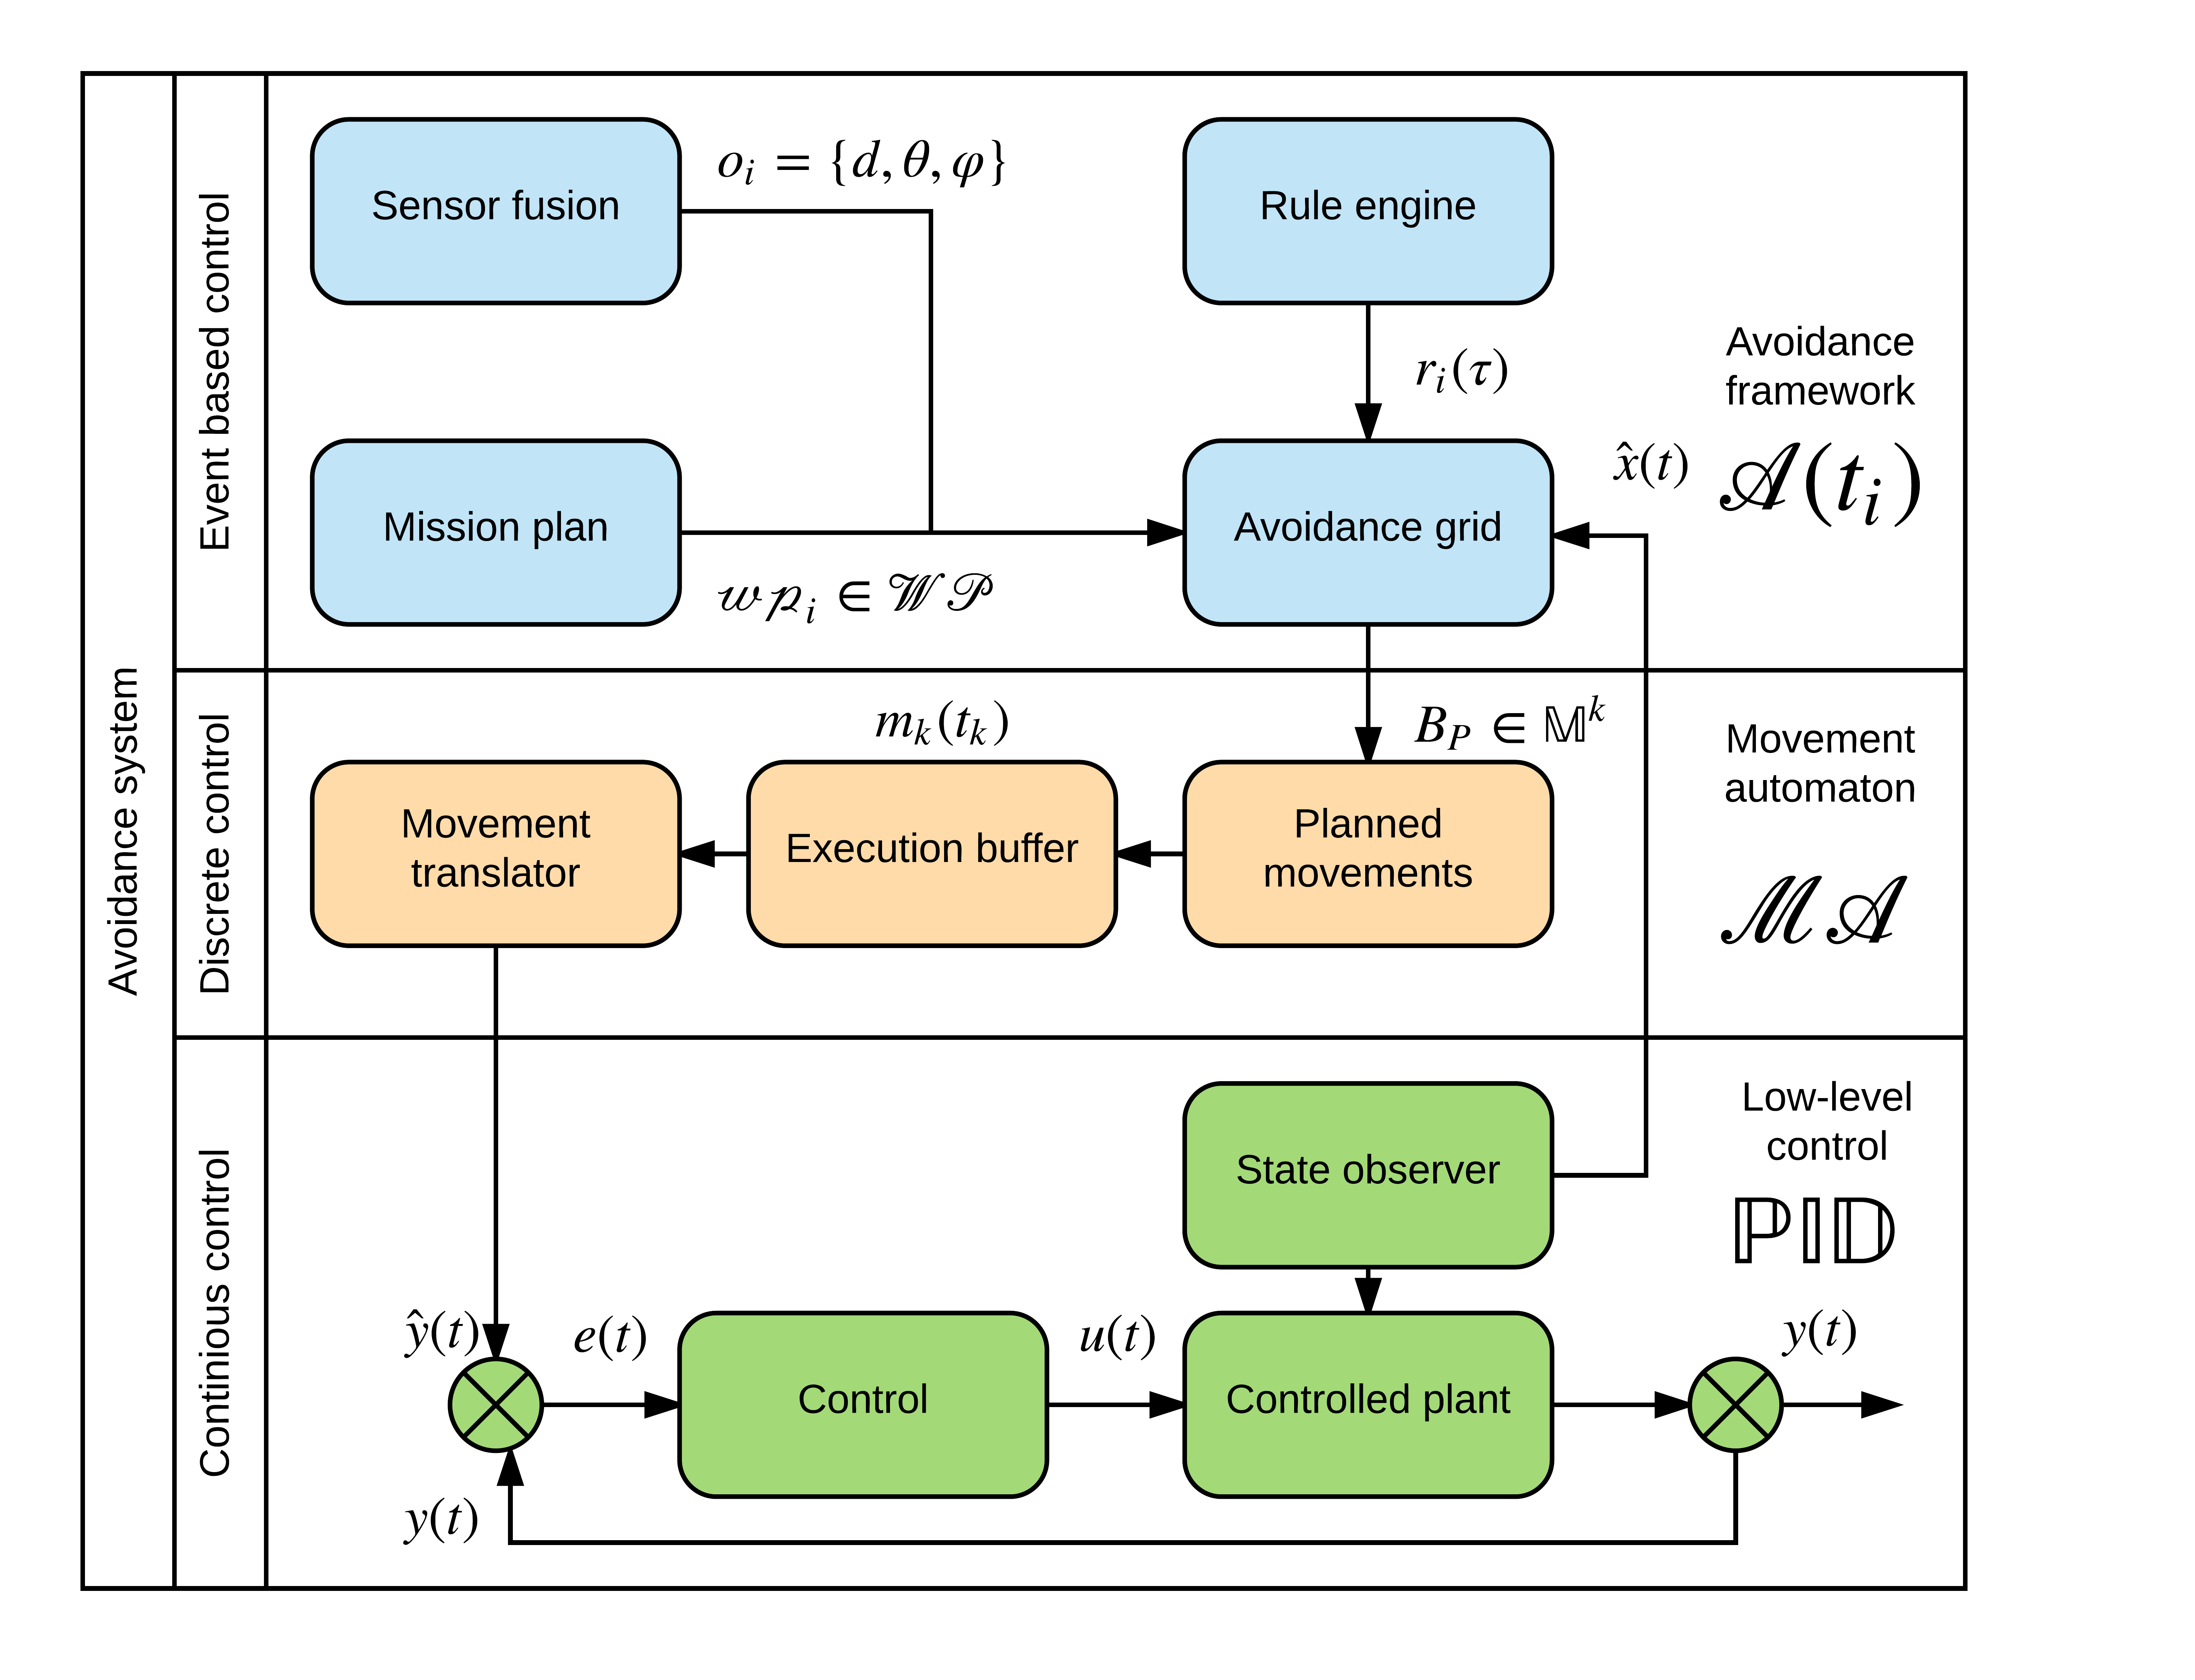
\includegraphics[width=0.8\linewidth]{\FIGDIR/TE001BlockSchemeOfControlConcept} 
    \caption{Obstacle avoidance based on Reach sets concept.}
    \label{fig:avoidanceConcept}
\end{figure}

\section{(R) Movement Automaton}\label{s:movementAutomatonTheory}

\paragraph{Idea:} The key idea is to create \emph{interface} between \emph{controlled plant} (UAV) and \emph{Avoidance Algorithm} to ensure \emph{Concept Reusability} at maximum degree.  The concept is following:

\begin{enumerate}

    \item \emph{Interface consumes} discrete command chain and guides UAS along \emph{desired trajectory}.
    
    \item \emph{Interface} can be used to \emph{predict trajectory} based on \emph{initial state} and future command chaining. 
\end{enumerate}

Frazolli provided the concept of \emph{Movement Automaton} (def. \ref{def:movementAutomaton}) a specialized type of \emph{Hybrid Automaton} (eq. \ref{eq:hybridAutomaton}), the concept is taken from his works \cite{frazzoli2001robust,frazzoli2000trajectory}. Other aspects and similarities are discussed over this chapter. 


\paragraph{Architecture:} The Movement Automaton can be seen as a consistent hierarchical abstraction of the continuous dynamics, in the sense outlined in \cite{pappas2000hierarchically}: \emph{Any sequence of movement primitives generated by the Movement Automaton results by construction in a trajectory which is executable by the full continuous system. We will give a deeper meaning to hierarchical consistency}. The implementation of our movement automaton is given in (fig.\ref{fig:avoidanceConcept}). 

\paragraph{Optimal Path Generation:} If the maneuvers are instantaneous (i.e. the UAS can transition instantaneously between two different trim trajectories), Reduction of stronger results obtained by Dubins \cite{dubins1957curves} and Reeds \cite{reeds1990optimal} concerning optimal paths for kinematic cars on the plane (see also \cite{soueres1998optimal}). 

\paragraph{Controllability:} The systems controlled by Movement Automaton (as in \cite{lavalle1998rapidly}), is controllable according to our definition, even though it is not
small-time controllable \cite{sussmann1983lie}.

\paragraph{Other Properties:} The other properties of movement automaton, like \emph{Stability, Robustness} and other important control properties are proven in \cite{frazzoli2001robust}.



\paragraph{Example:} The \emph{example} is given in (fig. \ref{fig:movementAutomatonExampleTheory}). The \emph{States} (Barrels) are connected by \emph{Transitions} (green arrows).

\emph{Hover} is neutral and \emph{initial} state, in this place the UAS stays on place and maintains altitude.

\emph{Forward flight} is when \emph{UAS} is flying in frontal direction with constant speed. The speed-up and slow-down is incorporated in \emph{Transition} between \emph{Hover} and \emph{Forward flight} states and its takes some time to execute. \emph{Transitions} between Turning states and \emph{Flight forward} state are almost instant. 

\emph{Steady turn left/right} is when \emph{UAS} is flying in frontal direction and starts steady turning left or right. 

\begin{note}
UAS in (fig. \ref{fig:movementAutomatonExampleTheory}) ignores the vertical maneuvering and it is expected to fly on horizontal plane.
\end{note}


\begin{figure}[H]
    \centering
    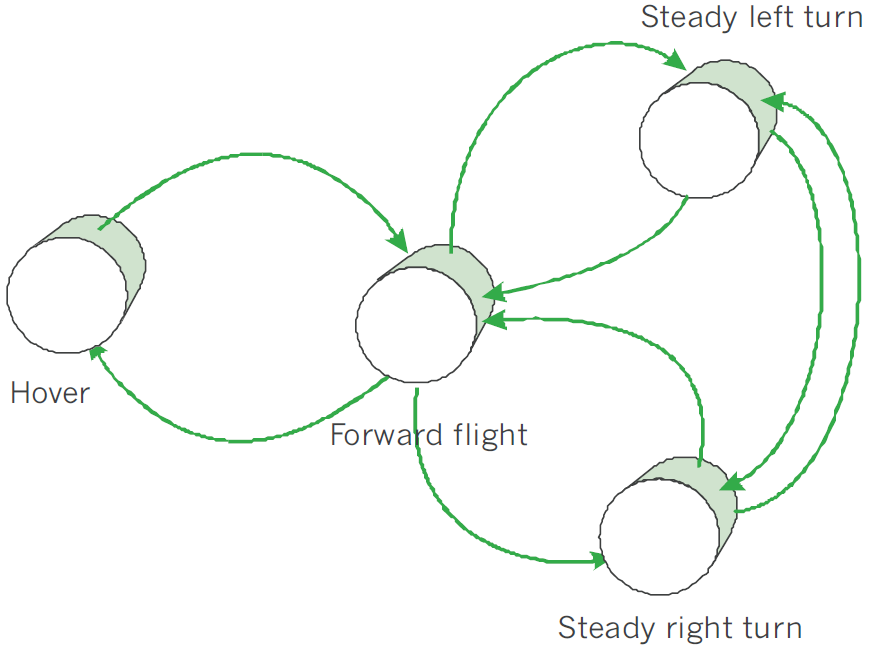
\includegraphics[width=0.55\linewidth]{\FIGDIR/TE030MovementAutomatonFrazzCite} 
    \caption{Movement Automaton for Copter UAS \cite{frazzoli2001robust}.}
    \label{fig:movementAutomatonExampleTheory}
\end{figure}

\paragraph{Used concepts:} The movement automaton is essential part of this work. Supporting the idea, that \emph{Obstacle avoidance framework} can be platform independent. 

The \emph{Movement Automaton} is used as is (sec. \ref{s:MovementAutomatonDefinitionAndProperties}). The implementation is described in (sec. \ref{s:modelMAImplementation}). The testing configuration was given in (tab. \ref{tab:testMovementOrientations}).


\section{(R) Sensor (Data) Fusion - Input Interface}\label{s:dataFusionProbabilisticModelTheory}
\paragraph{Idea:}  There is \emph{Need for abstract representation} of \emph{operational space}, which is independent of used sensors, technologies, information sources. The universal obstacle avoidance system should have \emph{portability property}. Our previous work \emph{Obstacle avoidance framework based on reach sets} \cite{gomola2017obstacle} have introduced similar concept of \emph{control interface}.

The original concept was using cell status interpretation, which was hardwired to LiDAR technology.  The new demand is to incorporate concepts of \emph{visibility}, \emph{reachibility} and \emph{obstacle probability}. The base methodst for \emph{Statistical Sensor Fusion} were outlined in \cite{gustafsson2010statistical}.

\paragraph{Key Concept:} \emph{Data fusion interface} (sec. \ref{s:dataFusionDefinition}) - interface to fuse sense data from various online, offline, cooperative, non-cooperative sources into single scalable {space and trajectory evaluation procedure}.
    
\paragraph{Related work:} \noindent UAS specific sensor fusion has been proposed by Ramsay in \cite{ramasamy2014avionics}. \emph{Next generation avoidance concept} \cite{ramasamy2014next} is introducing concept of higher level sensor fusion called \emph{data fusion}. 

The uncertainty and properties in \emph{Remotely Piloted Systems} have been discussed in \cite{chynchenko2016remotely}. The work provided concept of various performance ratings like visibility and obstacle rating, more details have been given in \cite{shmelova2016modeling}. This ratings were modeled only for operator decision making \cite{kharchenko2017modelling}, results are usable for automated decision making and space assessment. 

\emph{Probabilistic trajectory assessment} has been firstly proposed in \cite{kim2007uav} where trajectory was tracking and predicting \emph{safety properties} along. 

\emph{Game theory} viewpoint is firstly used in \cite{vidal2002probabilistic}. Probabilistic path planning using safety zones similar to cell classification of this work have been used in \cite{pfeiffer2005path}.

Probabilistic path search similar to our reach set representation using rapidly exploring path trees have been used in \cite{kothari2013probabilistically,blackmore2006probabilistic}. Relationship between classic grid search and probabilistic lattice search have been established in \cite{lavalle2004relationship}. A probabilistic approach for trajectory estimation via reduced lattice search is known from 1986 from work of Gessel \cite{gessel1986probabilistic} lattice paths were enumerated via movement sequences and similar technique is used in our reach set estimation method using movement automaton.  Pruning methods comparison and complexity can be found in \cite{esposito1997comparative}.

Overall concepts of probabilistic sets have been given by Hirota in \cite{hirota1981concepts}.  Free flight safety rating similar to our reachability concept have been presented in \cite{hoekstra2002designing}.

\paragraph{Shortcomings:} 

\begin{enumerate}
    \item \emph{Hierarchical calculation} - there is need to calculate \emph{avoidance trajectory} for incremental constraint applications. For example:
    \begin{enumerate}[a.]
        \item Calculate \emph{Minimal escape path} covering physical obstacles and intruders.
        \item Apply next level of constraints, like airspace restrictions and some virtual constraints. Then calculate path if exists, continue.
        \item Apply nice to have constraints, like non lethal weather, recalculate path.
    \end{enumerate}
    
    \item \emph{Source Reliability Evaluation} -  reliability evaluation is empirical process usually done by hand. The result aggregation is not standardized. There can be multiple sources of same rating, for example visibility, which needs to be aggregated into one.  
    
    \item \emph{Ambiguous rating definition} - There is multiple definitions especially for \emph{Reachibility rating} in works \cite{kothari2013probabilistically,blackmore2006probabilistic,gessel1986probabilistic}.
    
\end{enumerate}

\paragraph{Improvements in Our Work:}

\emph{Hierarchical calculation} is addressed in \emph{Mission Control run} (sec: \ref{s:missionControlRun}) where threats are hierarchically applied based on \emph{severity}.

\emph{Source reliability evaluation} is addressed in \emph{Static Obstacles} (sec. \ref{s:staticObstacles}) and \emph{Moving Obstacles} \ref{s:intruders}). The main rating for \emph{Detected obstacle, Map Obstacle} and \emph{Visibility} of space are established there. 

\emph{Clear rating definition} - the \emph{Reachibility} of space portion and \emph{Safety} rating for trajectory are established in \emph{Avoidance Grid Run} (sec. \ref{s:aviudabceGridRun})



\section{(R) Navigation Algorithms}\label{s:NavigationAlgorithms}
\paragraph{Idea:} The basic idea is to provide hierarchical\emph{navigation frame} with \emph{some optimal path search capabilities}. 

\paragraph{Standard Navigation:} The standard navigation is given as \emph{expected cost optimization problem} for \emph{future cost function} (eq. \ref{eq:costFunctionReachable}). The key concept of navigation algorithm was fully taken from \cite{gardi2018multi}. The decision was made based on navigation survey \cite{goerzen2010survey}. The \emph{descent} for landing is out of scope in this work, can be found in \cite{lim2018energy}. The navigation principle is roughly described in (sec. \ref{s:missionControlRun}).


\paragraph{Maze Solving Capabilities:} The \emph{maze solving capability} is usable in \emph{controlled airspace} where 2D maze solving algorithms are applicable. The notable implementation was for \emph{micro mouse robot} based on right hand rule \cite{mishra2008maze}. Flood fill algorithm is partially usable for 3D environment \cite{elshamarka2012design}. The application of \emph{maze solving} was given in case study \cite{chatelais2014maze}.

\paragraph{Hybrid Automaton Path Planning:} A hybrid automaton path planing based on $A*$ algorithm was given by Richards in \cite{richards2004hybrid}. The key idea was to use \emph{hybrid automaton} (eq. \ref{eq:hybridAutomaton}) as a reference generator. This idea was taken and formulated as \emph{Movement Automaton Predictor mode}. 

The similar idea where \emph{potential fields} were used as \emph{intruder model} and path was re-planned  based on events is given in \cite{dong2011hybrid}.

\paragraph{Mode Switch:} The \emph{Mode Switch Control} idea has been presented in \cite{ryan2005mode}. There were definition of behavioural switch between:
\begin{enumerate}
    \item \emph{Navigation Mode} - navigation control and behaviour was used.
    \item \emph{Task Specific Mode} - mode specific for tasks, authors were using modes for search and rescue. 
\end{enumerate}

This concept will be reused, the \emph{Task specific mode} will be \emph{Emergency Avoidance Mode} in Our case. The triggering events and switch conditions will be defined in (sec. \ref{s:missionControlRun}).

\paragraph{Used concepts:} The \emph{Following concepts} were used in navigation loop:
\begin{enumerate}
    \item \emph{Standard navigation} taken from \cite{gardi2018multi} minor implementation changes using offline optimization. The purpose of navigation loop is to bring us closest to the waypoint, if its reachable. Navigation example (sec. \ref{s:testRuleMixed}).
    
    \item \emph{Maze solving capabilities} partially taken as secondary functionality based on \cite{elshamarka2012design}. The purpose is the \emph{looping prevention}. The example was given in (sec. \ref{s:testMaze}) .
    
    \item \emph{Mode switch} partially taken as main feature from \cite{ryan2005mode}, the triggering events were identified and defined by author and can be found over (chapter \ref{ch:approach}).
\end{enumerate}


\section{(R) Reach Set Estimation}\label{s:ReachSetEstimationTheory}
\paragraph{Idea:} The basic idea for \emph{Discrete Reach set Estimation  method} is taken from \cite{ljungqvist2017lattice}. The focus of their work is to generate paths that are kinematically feasible. Path following controllers in order to find techniques to stabilize the system around these paths \cite{ljungqvist2016path,evestedt2016path}. 

Lattice-based planners have been deployed with great success on several robotic platforms \cite{pivtoraiko2009differentially,urmson2008william,cirillo2017videogames,tomlin2000game,chen1997game}. However, a problem with lattice-based approaches is the exponential complexity in the dimension of the state space which can limit the use for more complicated models.

The optimization problem was solved real-time by \emph{Avocado solver} \cite{houska2011acado}.

\paragraph{Example:} The \emph{example of movement lattice} is given in (fig. \ref{fig:latticeMovementPrimitivesExample}). Truck (black rectangle) is towing Trailer (red rectangle). The \emph{state} have only one \emph{reach set impacting variable} - \emph{trailer displacement}. When trailer displacement is $0^{\circ}$ (fig. \ref{fig:noDisplacementLattuce}) the lattice representation of \emph{Reach Set} is different that in case of small left/right tilt (fig. \ref{fig:displacementleftrightlattuce}).

\begin{figure}[H]
    \centering
    \begin{subfigure}{0.48\textwidth}
        \centering
        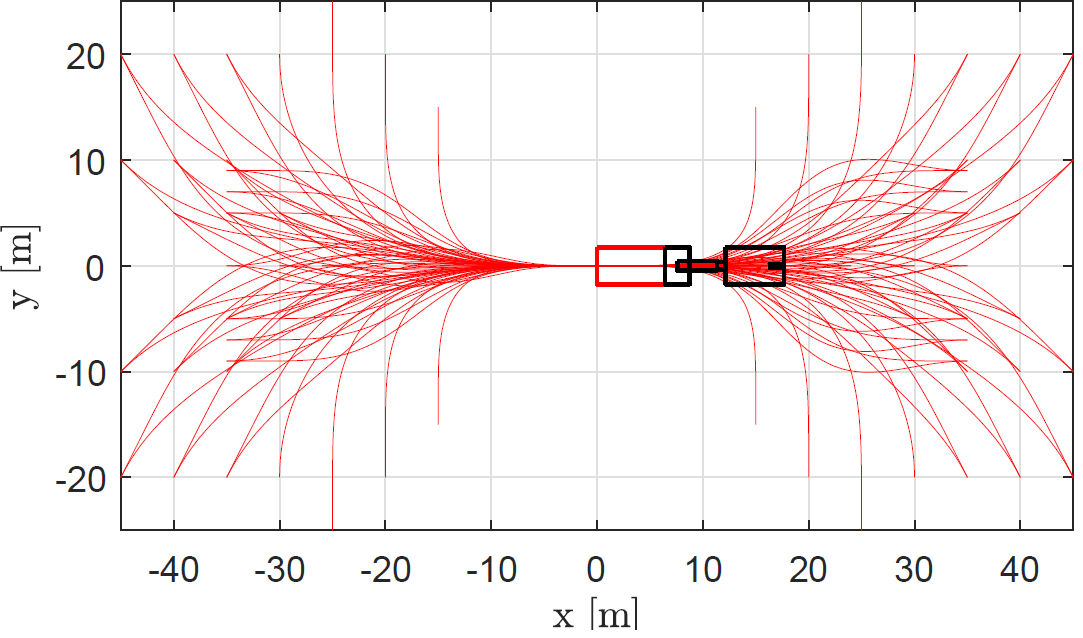
\includegraphics[width=0.9\linewidth]{\FIGDIR/TE028LattuceMovementSet01}
        \caption{Trailer displacement $0^{\circ}$.}
        \label{fig:noDisplacementLattuce}
    \end{subfigure}
    \begin{subfigure}{0.48\textwidth}
        \centering
        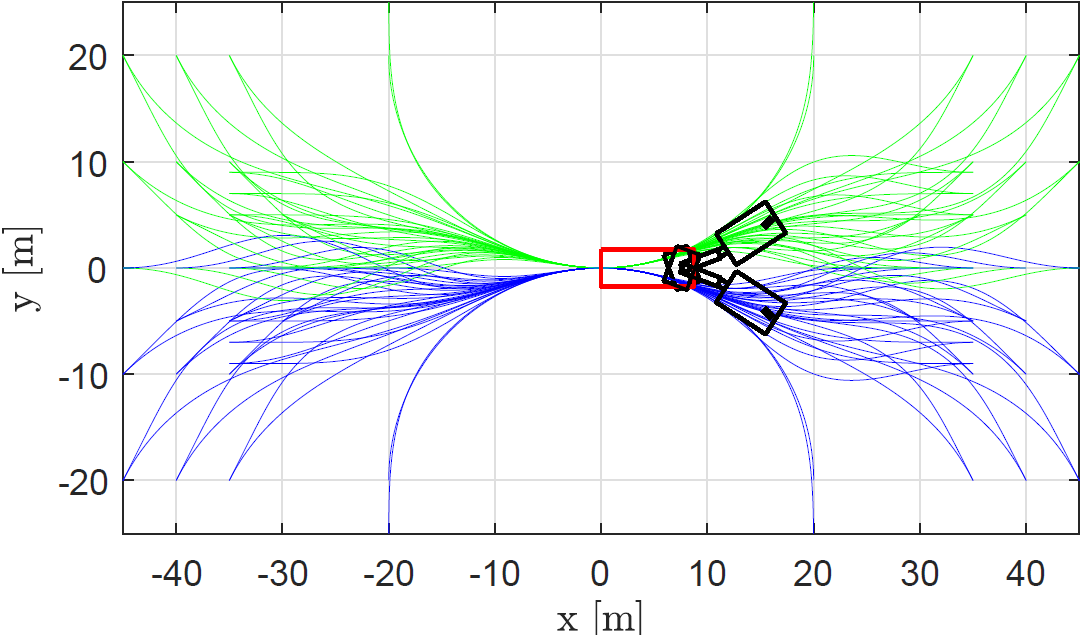
\includegraphics[width=0.9\linewidth]{\FIGDIR/TE029LattuceMovementSe02t} 
        \caption{$12^{\circ}$ (green) $-12^{\circ}$ (blue).}
        \label{fig:displacementleftrightlattuce}
    \end{subfigure}
    
    \caption{\emph{Movement set primitives} for Lattice Based Movement Planning. \cite{ljungqvist2017lattice}. }
    \label{fig:latticeMovementPrimitivesExample}
\end{figure}

\paragraph{Benefits:} Presented method of \emph{Lattice Search}  is  de-facto \emph{Reduced Reach Set Approximation} in open space for \emph{Truck-Trailer} system. 

The idea of \emph{Movement primitives} is very close to \emph{Movement Automaton} (def. \ref{def:movementAutomaton}), which can be used as \emph{control interface} effectively. 

The \emph{Constraints} of obstacle set in \emph{Known world} (sec. \ref{s:KnownWorld}) are supported to some degree.

\paragraph{Shortcomings:} There are following shortcomings which were identified in this approach:
\begin{enumerate}
    \item \emph{Limited system dimension} - given method works in \emph{real time} only if dimension of \emph{system state space} does not exceed $4^{th}$  rank.
    
    \item \emph{Real time optimization} - real time optimization is main cause of \emph{limited system dimension}. If the decision time can be discrete (which movement automaton enforces) then offline optimization  can be used. 
    
    \item \emph{Continuous space disparity} - the example (fig. \ref{fig:latticeMovementPrimitivesExample}) shows there are member variables of \emph{State Space} which significantly impacts the shape of lattice (reach set estimation). This is not a problem in real-time environment. The discretization of \emph{Time domain} raises this as a shortcoming.
    
    \item \emph{Trajectory Tracking} - approach generates \emph{Continuous Domain} reference signal. For \emph{Discrete Domain} it is necessary to address this issue.
\end{enumerate}

\paragraph{Improvements in Our Work:}

\emph{Limited system dimension} - the discretization due the higher system dimension and  increased maneuver complexity goes hand-in-hand with \emph{pre-calculation} of the \emph{Reach Set}. This shortcoming is addressed in (sec. \ref{s:constrainedTrajectoryExpansion}).

\emph{Real time optimization} -  replaced by \emph{Discrete offline optimization problem}. The \emph{general cost function} is given in (eq. \ref{eq:costFunctionReachable}). The optimization problem solved in this work is defined in (eq. \ref{eq:trajectoryTrackingOptimalizaitonProblem}).

\emph{Continuous space disparity} - The \emph{pre-calculated reach set estimation} can be valid with small \emph{marginal error} for some region in \emph{system state space}. The dynamic method for state space segmentation can be used \cite{takahashi1996reasonable}. This aspect is not addressed in this work, because it is strongly depending on the system behind movement automaton. 

\emph{Trajectory Tracking} - The \emph{movement automaton} (def. \ref{def:movementAutomaton}) in Control Mode can be used to track reference trajectory in form of \emph{Movement Buffer}(def. \ref{def:MovementBuffer}). Other option is to use \emph{thick waypoint trajectory tracking for UAV} like in \cite{kaminer1998trajectory} or \cite{murillo2015generalized}. The work will use only \emph{Movement Automaton} as controller/predictor. 




\section{(R) Testing Framework}\label{s:TestingFrameworkTheory}

\paragraph{Idea:} \emph{Reuse LSTS toolchain architecture} for DAA testing framework.

\paragraph{LSTS Toolchain:} Software architecture used in modern unmanned aerial vehicles must be system independent and scalable. Writing own control software for unmanned aerial vehicle and ground station is unthinkable in current state of art.  Most notable framework for unmanned aerial vehicle development is LSTS tool chain from University of Porto \cite{merani2011underwater}. This tool chain is widespread in other universities and multiple independent applications are based on it \cite{rajan2013towards}.

\begin{figure}[H]
    \centering
    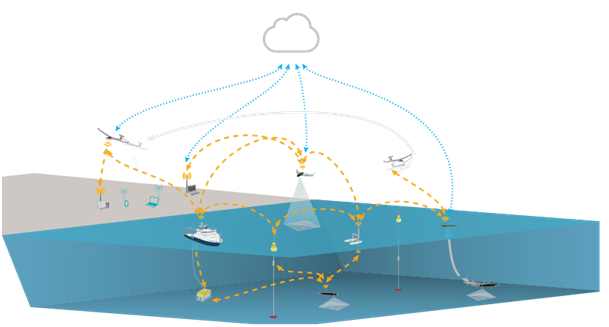
\includegraphics[width=0.9\linewidth]{\FIGDIR/TE036LSTSDeployment}
    \caption{Example of LSTS toolchain deployment in real environment \cite{pinto2006neptus}}
    \label{fig:lstsdeployment}
\end{figure}

Example of software architecture implementation is shown in figure \ref{fig:lstsdeployment} LSTS HUB (cloud iconography) is collecting all important data from currently executing missions. Data are transferred via REST API (dotted blue lines) to HUB.  Commanded vehicles can be unmanned copters, planes, ships, submarines or floating sensors compounds. Each vehicle has installed DUNE which is responsible for vehicle command and ground control station communication. Deployment, range of command and status messages can vary. Ground station can be implemented on personal computer (any platform) in NEPTUS environment or mobile platform (Android OS) in ACCU environment. Ground station environments are customizable and open source. Layout of ground station can be customized to need of current mission via plugins or console configuration. Vehicles and ground stations are communicating via IMC protocol (orange dashed lines). Communication channel is platform independent.


\textit{Glued} is a Debian-based open source operating system which was initially released in 2010.  Over the years it has become fairly widespread and been provided continuous updates.  Meanwhile, a notable development community has emerged, where advice and support can be received as more applications are investigated. Some of the merits of the operating system are its reliability and customizability. Operation system is developed for unmanned autonomous vehicles. It is widely used in air, sea and land vehicles. Customization allows the operating system to be tailored to the specific usage. For this purpose, this includes stripping off functionality which is not required, thus releasing resources to be focused on the essential tasks. Glued is the operating system favored by the Beaglebone development community, and thus there exist considerable amounts of helpful documentation for this set-up.

\textit{DUNE: Unified Navigational Environment} is an on-board software solution for unmanned vehicles. Multiple applications already run on this software. Almost any extension can be added to this to this environment. The software solution provides means for interacting with the connected components as well as control, navigation, supervision and plan execution.  It is both CPU architecture independent and OS independent.  It is written in C++ and developed by LSTS: Underwater Systems and Technology Laboratory.

\textit{Neptus} \cite{pinto2006neptus,dias2006mission,dias2005neptus} is a command and control software operated from a ground station. It is designed to operate well together with Dune and was also developed by LSTS. Neptus provides tools for remotely monitoring UAVs and assigning plans and commands in real-time missions, supporting multiple connections dynamically. Furthermore, it provides possibilities for both simulating missions and reviewing previously performed operations. This is presented in a customizable interface equipped with map layers and control panels. It is written in Java and available for both Windows and Linux systems.

The \textit{Inter-Module Communication} \cite{martins2009imc} (IMC) protocol was developed by LSTS to provide reliable communication between the systems.  The protocol is message-oriented, such that messages can be sent and received from a bus which connects independently run threads or systems.  Thus it functions as a method of communication between tasks internally in Dune, and can also be passed to and from other vehicles or computers running Dune or Neptus.  IMC is platform independent at multiple messages have been already developed and supported by both DUNE and Neptus (around 400 status/command messages).

\textit{HUB} is communication hub for data dissemination and situation awareness. This module is responsible for complex mission execution, when cooperation of multiple pilots/vehicles is required. This module can be imagined as airport tower center, which is monitoring all flights in airport (operation site) area. This tool implements REST API for communication between various ground stations and operating vehicles.

\paragraph{Movement Automaton Control} Marconi used \emph{hybrid automaton} with forced \emph{State Switch} via buffer \cite{marconi2009control}. The key concept is that \emph{Automata} state switch is forced as \emph{external source command}. Our \emph{Movement Automaton} implementation know only \emph{forced state switch} like in \cite{frazzoli2000trajectory}. 

\paragraph{Used concepts:} Most of the architecture was re-used in our approach, the concept of \emph{Rule engine} (sec. \ref{sec:ruleEngine}) was introduced to cover missing \emph{UTM} related functionality. The implementation in Matlab was influenced by Alessandeti works \cite{allesandeti2016virtualArena,alessandrettinotes}. The other aircraft dynamic and control related concepts were taken from  \cite{stevens2015aircraft}.

\section{(R) UTM Services}\label{s:utmServicesTheory}
\paragraph{Idea:} Take the Airbus UTM concept \cite{airbusUTM2018blueprint} combine it with \emph{EUROCONTROL} concept \cite{andrewhately2018} to obtain legal framework. \emph{Provide conflict resolution functionality} for \emph{Controlled Airspace}:
\begin{enumerate}
    \item \emph{Collision Detection} - define minimal required functionality for collision detection.
    \item \emph{Collision Resolution} - implement \emph{Rules of the Air} \cite{standard1986recommended}.
\end{enumerate}

The \emph{implementation} of \emph{UTM services} described in (sec. \ref{sec:UTM}) is given in (sec. \ref{sec:UASTrafficManagement}).

\paragraph{UTM Operation Modes:} \emph{defined in } \cite{airbusUTM2018blueprint} are following:
\begin{enumerate}
    \item \emph{Free route} (fig. \ref{fig:UTMFreeRouteMode}) is when aircraft can fly any path, so long as their planned path is coordinated with and de-conflicted from the paths of other aircraft by a traffic manager and approved based on calculated risk. Free routing is being introduced worldwide, such as free route airspace. This allows commercial flights to freely plan their route through participating sectors during cruise. There is less freedom for an aircraft in this situation than in basic flight, since its request may be rejected.
    
    \item\emph{Corridors} (fig. \ref{fig:CorridorMode})  are defined volumes in space, useful for managing airspace in high demand or to manage traffic flow and separation. Coordination is necessary to ensure safety in this airspace. A corridor may take on many different shapes. Aircraft are often guided inside corridors using predetermined routes analogous to approach procedures used worldwide today.
    
    \item\emph{Fixed route} (fig. \ref{fig:fixedRoute}) are used to ensure safety when there is high traffic density or in any location where structure is required to ensure safe operations. This could include locations such as airports or warehouses. These routes could be constructed or modified dynamically based on calculated risk. The most restrictive version is a predetermined path, where the only variable is when an aircraft is at a specific point in the path.
\end{enumerate}

\begin{figure}[H]
    \centering
    \begin{subfigure}{0.32\textwidth}
        \centering
        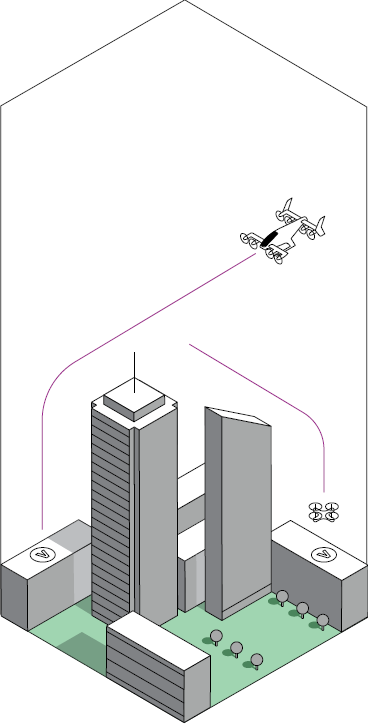
\includegraphics[width=0.9\linewidth]{\FIGDIR/TE032FreeRoute}
        \caption{Free route.}
        \label{fig:UTMFreeRouteMode}
    \end{subfigure}
    \begin{subfigure}{0.32\textwidth}
        \centering
        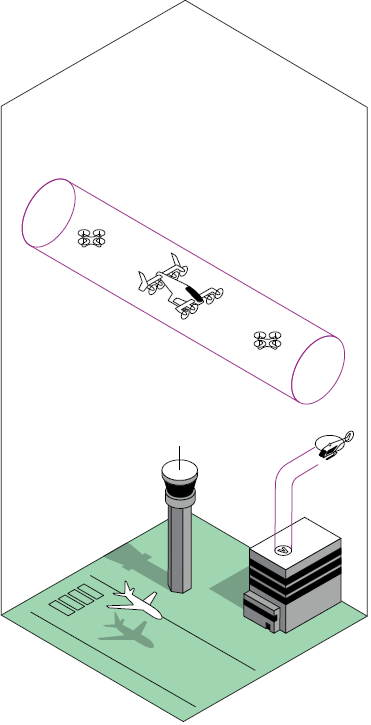
\includegraphics[width=0.9\linewidth]{\FIGDIR/TE034Corridors} 
        \caption{Corridors.}
        \label{fig:CorridorMode}
    \end{subfigure}
    \begin{subfigure}{0.32\textwidth}
        \centering
        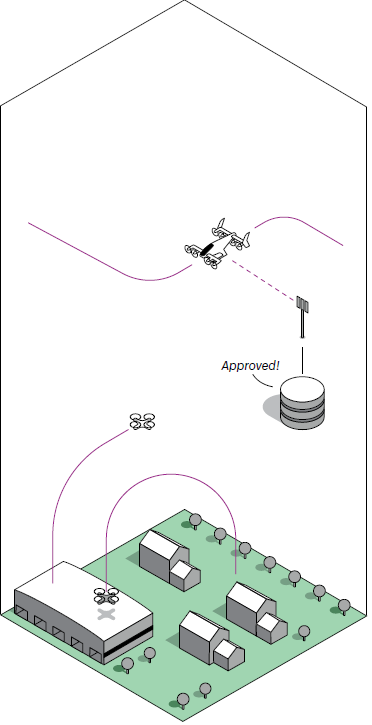
\includegraphics[width=0.9\linewidth]{\FIGDIR/TE035FixedRoute} 
        \caption{Fixed route.}
        \label{fig:fixedRoute}
    \end{subfigure}
    
    \caption{UTM Operation Modes.}
    \label{fig:utmOperationModes}
\end{figure}

\paragraph{Used Concepts:} The implementation of our UTM services  is focused on \emph{Free route mode} (fig. \ref{fig:UTMFreeRouteMode}). The \emph{Corridors} and \emph{Fixed routes} are just additional \emph{space/time constraints}.
    
	
%% This adds a line for the Bibliography in the Table of Contents.
\addcontentsline{toc}{chapter}{Bibliography}
%% *** Set the bibliography style. ***
%% (change according to your preference/requirements)
%\bibliographystyle{plain}
%% *** Set the bibliography file. ***
%% ("thesis.bib" by default; change as needed)
\bibliography{thesis}

%% *** NOTE ***
%% If you don't use bibliography files, comment out the previous line
%% and use \begin{thebibliography}...\end{thebibliography}.  (In that
%% case, you should probably put the bibliography in a separate file and
%% `\include' or `\input' it here).

\end{document}
